\documentclass[review]{elsarticle}
%\documentclass[final,times,letterpaper,12pt]{elsarticle}

\usepackage{lineno,hyperref}
\usepackage{graphicx} 
\usepackage{subcaption}
\usepackage{amsmath}
\usepackage{booktabs}


\usepackage[dvipsnames]{xcolor} % Für Einfärbung von Notizen. Sollte am Ende wieder entfernt werden.

\modulolinenumbers[5]

%\usepackage{etoolbox}
% \patchcmd{<cmd>}{<search>}{<replace>}{<success>}{<failure>}
%\patchcmd{\emailauthor}{(#2)}{}{}{}
\patchcmd{\urlauthor}{(#2)}{}{}{}

\journal{Journal of PLACEHOLDER}


%%%%%%%%%%%%%%%%%%%%%%%
%% Elsevier bibliography styles
%%%%%%%%%%%%%%%%%%%%%%%
%% To change the style, put a % in front of the second line of the current style and
%% remove the % from the second line of the style you would like to use.
%%%%%%%%%%%%%%%%%%%%%%%

%% Numbered
%\bibliographystyle{model1-num-names}

%% Numbered without titles
%\bibliographystyle{model1a-num-names}

%% Harvard
%\bibliographystyle{model2-names.bst}\biboptions{authoryear}

%% Vancouver numbered
%\usepackage{numcompress}\bibliographystyle{model3-num-names}

%% Vancouver name/year
%\usepackage{numcompress}\bibliographystyle{model4-names}\biboptions{authoryear}

%% APA style
\bibliographystyle{model5-names}
\biboptions{authoryear}

%% AMA style
%\usepackage{numcompress}\bibliographystyle{model6-num-names}

%% `Elsevier LaTeX' style
%\bibliographystyle{elsarticle-num}
%%%%%%%%%%%%%%%%%%%%%%%

\begin{document}

\begin{frontmatter}

\title{PLACEHOLDER Title}

\author {Jasper Bär\corref{cor1}}
\ead{ja.baer@stat-econ.uni-kiel.de}
\ead[url]{PLACEHOLDER Github url}

\cortext[cor1]{PLACEHOLDER}

\begin{abstract}
PLACEHOLDER Abstract
\end{abstract}

\begin{keyword}
PLACEHOLDER Keyword 1 \sep Keyword 2 \sep Keyword 3 \sep Keyword 4 \sep Keyword 5
\end{keyword}

\newpageafter{abstract}

\end{frontmatter}

%\linenumbers

\section{Introduction} \label{sec:intro}

Central bank communication has become an important tool of modern monetary policy \citep{Blinderetal2017}. Central banks use communication as an important tool for guiding inflation expectations and ensuring trust. In recent years, most of the communication was aimed at financial experts. However, central banks are increasingly reaching out to the general public \citep{Blinderetal2022}. The media plays a crucial role in this mechanism by making the information of the central bank communication available to the general public, which makes it crucial to understand how central bank communication is reported in the media for understanding the effects of central bank communication on the general public.
\\
Most of the literature focuses on a direct link between central bank communication and financial variables. \textcolor{red}{(To close to \cite{Picaultetal2022}.)} Similar to \cite{Picaultetal2022}, I adapt a framework by \cite{HayoNeuenkirch2015} where media acts as a channel between the central bank communication and the perception of monetary policy by financial markets. 
Following this line of thought, I assume that the media coverage of central bank communication acts as a channel between the central bank and the households. I assume that households consume the news about the central bank communication rather than the original central bank communication. This view is in line with \cite{Gardt2022} who show that according to the ECB Knowledge and Attitudes Survey, May 2021 households mostly hear about the ECB from television and newspapers (online and printed) and rarely by using direct sources like the ECB website. \textcolor{red}{(To close to \cite{Blinderetal2022}.)}
\\
Since \cite{Carroll2003} created a model for inflation expectations that considers the amount of media coverage several studies have analyzed the role of media coverage for the inflation expectation forming process \cite{Ehrmann2017},  \textcolor{red}{(To close to \cite{Larsen2021}, more citations?)}
Newer studies, extend the analysis to also incorporate the tone \citep{LamlaLein2014} and the topics \citep{Larsen2021} of media coverage. 
\\
Using the \textcolor{red}{data-driven} lexicon approach by \cite{PicaultRenault2017}, I find that news and ECB communication is strongly correlated with the current inflation in Germany with a few noticeable exceptions. Furthermore, the \textcolor{red}{idiosyncratic} error from a linear regression of media coverage on ECB communication is strongly correlated with the inflation expectation gap of German households.
\\
%This view gets supported by a number of survey-based studies indicating that household are often poorly informed about monetary policy and the objectives of their respective central banks. \cite{Cruijsenetal2015} show that Dutch households understanding about the ECB's objectives are poor. Similar most German \citep{HayoNeuenkirch2018} and Italian \citep{Bottonetal2021} households do not know that the main objective of the ECB is to maintain price stability in the euro zone. However, \cite{Cruijsenetal2015} and \cite{HayoNeuenkirch2018} show that people who receive their information about monetary policy via television and newspapers are better informed their central bank and monetary policy.\textcolor{red}{(To close to Blinder et al. 2022)}
%nochmal nachprüfen
%However, \cite{Picaultetal2022} and \cite{Cruijsenetal2015} note that the perception of financial markets is simultaneously influenced by the central bank communication and the media coverage of the corresponding events and central bank communication.
%A small but rapidly growing branch of the literature focuses on central bank communication, i.e., the information provided by central banks to the general public, and its connection to different variables of interest like financial variables or future monetary decisions of the central bank. For example, \cite{PicaultRenault2017} show that ECB press statements can be used to predict future ECB monetary decisions. \textcolor{red}{(Give more examples)}
%A subbranch of this literature focuses on the connection between inflation expectations and central bank communication. \cite{Picaultetal2022} investigate how the reporting about the ECB in the media can be used to predict financial market inflation expectations. \\
% Kurzer Abschnitt um Newspapers zu rechtfertigen (siehe Blinder et al. 2022)
% Kurzer Abschnitt in der ich auf Media Biases eingehe (Media reacts to central bank communication, negativity bias)
I investigate the influence of media coverage in German newspapers of ECB press conferences on household's inflation expectation accuracy. 
Firstly, I investigate if the information given in regard to inflation in media coverage deviates from the inflation information in the original press conferences by the ECB which would introduce a bias and could potentially influence how the general public perceives monetary policy decisions. Secondly, I investigate how media coverage and central bank communication can be used to \textcolor{red}{explain} the household's inflation expectation errors.
\\
This paper is to my knowledge, the first paper which explicitly investigates the link between ECB communication and news coverage in regard to household inflation expectations. Furthermore, it contributes to the literature by demonstrating how the news about inflation deviates from the corresponding ECB communication, allowing us to better understand how the ECB communication is conveyed to the general public and explains the channel through which the general public reacts to ECB communication.
\\
\\
% Furthermore, this paper applies a semi supervised approach that does only rely on a few pre-selected words instead of a full training dataset.
\textcolor{red}{(NOTE 1: I could maybe ask Tri and take his method instead. It is still supervised, but I could slightly modify it to produce a lexicon. It would most likely be an improvement over Picault et. al (2017) due to the word embeddings)}
\textcolor{red}{(NOTE 2: Before I can describe the model which I use for the second part, I need to certain what exactly I want to regress and how to do it.)}
\section{Data} \label{sec:Data}

My dataset consists of two different parts. The textual data from the ECB and the Media and the quantitative data regarding inflation and inflation expectations. In  section~\ref{sec:Textual Data} I describe the textual data. In section~\ref{sec:Text Classification} I describe how I transformed the textual data into quantitative data and in section~\ref{sec:Quantitative Data} I describe the remaining quantitative data.

\subsection{Textual Data} \label{sec:Textual Data}

I collected two separate datasets for the textual analysis, one for the ECB communication and one for the media news.
The ECB’s main channel for communication to the media are their press conferences \textcolor{red}{(CITE?)}. The press conference takes place after the ECB’s Governing Council took their monetary policy decision every six weeks. I collected ECB press conference from 2000 until 2022 with a webscrapper from the official ECB website \footnote[1]{The press conferences can be found under https://www.ecb.europa.eu/press/pressconf/html/index.en.html}. I discarded the Q\&A section and all sections which carry no significance, like greetings and acknowledgments, leaving only the introductory statements \textcolor{red}{(cite other who done it similarly)}.
\\
\\
\textcolor{red}{PLACEHOLDER Description of News Dataset}
\\
\\
\textcolor{red}{Note 1: Before I can do the description of the news dataset, I need to know which data I am allowed to use. The next part describes how I clean the news dataset}
\\
\textcolor{red}{Note 2: News dataset is in German, ECB dataset in English}
\\
To filter out any data that is not relevant for inflation, I only included sentences which contain the word “Inflation” (inflation) and synonyms of inflation like “Preisteigerung” (price increase). Furthermore, I filtered out all purely financial news, like reporting of stock movements or business news \textcolor{red}{(better word?)}.
\\
\textcolor{red}{Note 3: Provide list of synonyms somewhere ?}
\\
\textcolor{red}{Note 4: Not sure if this is the best way to select inflation related sentences. Maybe some kind of topic modeling would be better suited.}
\\
To reduce the dimensionality of the data I apply several pre-processing steps to the two datasets which are commonly used in the literature: Lowercasing, removing punctuation, removing stopwords (e.g., and, but, or) which carry no information and removing numbers.
\\
\textcolor{red}{NOTE 5: Currently the news dataset includes all inflation related sentences without differentiating between ECB and non ECB related news. I probably need to change that, but how do I do that and makes that even sense?}

\subsection{Quantitative Data} \label{sec:Quantitative Data}

%I use the quarterly year-on-year HCPI growth rate for the Eurozone collected from the Eurostat database as inflation.
The ECB surveys each quarter professional forecasters regarding their annual HICP expectations and provides the results to the general public. The survey ranges from the first quarter of 1999 up until the last quarter of 2022. I use the one-year-ahead annual HCPI point forecast averaged over all responds as my professional inflation forecast. 
\\
\textcolor{red}{NOTE: Besser wäre es, wenn ich Datastream benutze, um an Reuters Umfragedaten zu gelangen.}
\\
The consumer inflation expectation is based on the results from the monthly European Commission’s Business and Consumer Survey. The survey collects information about households inflation expectations by asking them if they expect that the prices increase more rapidly, increase at the same rate, remain unchanged or decrease in the next 12 months. To transform the qualitative survey answers into quantitative inflation expectations, I use the rolling-window regression based approach by \cite{Lahiri2015}. See \ref{sec:Quantification of Inflation Expectations} for an explanation.
\\
\textcolor{red}{NOTE: Change window size.}

\section{Text Classification} \label{sec:Text Classification}

In the following section I will lay out how I quantified the ECB communication and news. I do this by separating my dataset into individual sentences and then classify each sentence according to predefined categories. The ECB press conferences are classified into three categories where each category consists of three classes. The first two categories are taken from Picault et. al (2017). The first category describes the monetary stance expressed as monetary hawkish, monetary neutral or monetary dovish. The second category describes the economic outlook either as positive, neutral, or negative. I add a third class which describes the inflation outlook either as increasing, steady or decreasing. This third class allows for a direct comparison of the inflation expectations communicated in the ECB press conference to the inflation expectations expressed by the news media.
The News articles are classified into two categories where each category consists of three classes. The first category describes the economic effect of the inflation expressed in the news which can be either positive, neutral, or negative. The second category describes the inflation direction which can be either increasing, neutral or decreasing.

\subsection{Method for Quantifying the Central Bank Communication and News Coverage}

Two main approaches are mostly used for text classification, the lexicon-based approach, and the machine learning approach. For the lexicon approach a text is classified by taking a list of words, the lexicon, where each word belongs to one of the desired categories, such as “good” for positive sentiment or “bad” for negative sentiment. The text is classified by counting the occurrence of each of these word in the text. The lexicon approach can be modified by adding linguistic rules like negations \textcolor{red}{CITE?}.
\\ 
The machine learning text classification approach classifies a text based on supervised or semi-supervised models to a given category. In recent years, deep-learning models have been widely used for text classification.
\textcolor{red}{Continue this part with some examples}

\subsection{Training Dataset}
In the next section I will use supervised models to classify my data into several categories. I trained the models with two trainings dataset which I created, one for the news and one for the ECB press conference. I manually classified 3000 randomly drawn sentences from the ECB press conferences according to the three categories where each sentence was labeled with one of the three classes for each category.  Similarly, 3000 sentence were randomly drawn from the news corpus and labeled based on the two categories. The sentences were then used to classify the remaining sentences from my dataset with the method described in the next two sections.
\\
\textcolor{red}{Note 1: Is it obvious enough why I used two different training datasets?}
\\
\textcolor{red}{I should further describe my annotation scheme in the appendix and give some examples.}
\subsection{Lexicon Based Text Classification}
The simple implementation and transparency of Lexicon-based sentiment classification has made it widely used in the literature Shapiro (2020), (CITE), (CITE), (CITE), (CITE). Several lexicons exist for sentiment classification (CITE), (CITE), (CITE). However, these lexicons are not optimized for ECB communication or economic news. (FIND EXAMPLE). Picault et. al (2017) solve this problem by manually classifying each sentence in the ECB press conference based on their monetary stance and economic outlook. The classified sentences are then used to build a lexicon from the word used in the press conferences to classify the monetary stance and economic outlook of a press conference. I implement their approach with my own training dataset. The resulting lexicon is then used to classify each sentence in the ECB press conference for each of the three categories with the formula:
\textcolor{red}{Insert Formula}, same as in Picault et. al (2017) or any other similar papers. It’s just positive words – negative words divided by all words,)
with the class score s, the press conference i, the category c, the class j and the number of word occurrences n. A final score for each category in each press conference is calculated by taking the averaging the category score over all sentences from the corresponding press conference.
I slightly deviate from Picault et. al (2017) by first calculating the category score for each sentence instead of directly calculating score for the full press conference. My approach however is in line with most of the literature (Example from book or paper?).
Similiar to the press conferences, I calculate the category score for the news. First I create a lexicon for each of the two categories with the method from Picault et. al (2017). The category score for each news sentence in my dataset is calculated with (EQ). A monthly category score is calculated by averaging the sentence score for each month.
I further deviate from Picault et. al (2017) or similar papers like Marozzi (2021) (Still WP, and he at least uses valence shifters) by applying several linguistic rules to take grammatical(?) relations into account.
(I added negation handling and I will add some more rules. Not sure if I should describe that in the main text or in the appendix. The rules are using POS tags to identify negative and positive phrases, e.g., a negative adjective in front of a positive noun results in a negative phrase instead of a neutral phrase.

\section{Descriptive Analysis} \label{sec:Descriptive Analysis}

\subsection{News Indexes}\label{sec:News Indexes}

Figure~\ref{fig:News Index}(a) depicts the INI together with the monthly Germam CPI growth rate from 2000 to 2018. The index correlates with the inflation with the noticeable exception of the inflation decrease during the Great Recession which was not fully depicted by the INI. The low inflation phase from 2014 to 2016 was however accompanied by a dip of the INI which was lower than during the Great Recession. 
Figure~\ref{fig:News Index}(b) depicts quarterly German CPI growth from 200 to 2018 together with the number of sentences which I identified as inflation related divided by the total number of sentences to account for the varying number of articles in each year.

% I use this ration rather than the total number of words related to my topic of interest like most others e.g. (CITE) to take into account the varying number of articles in each year. The number of published articles steadily increased other the years.(CHECK, put that into Appendix?).

Before 2014 an increase in inflation related news is typically accompanied by a high inflation phase. However, from 2014 to 2017 the amount of inflation related news is high during the low inflation phase and remains alleviated afterwards. 
\\
\textcolor{red}{Note: Is there more to say?}

   \begin{figure}[h!]
    \centering
    \setkeys{Gin}{width=\linewidth,height=6cm} %set image parameters
\begin{subfigure}{6cm}
    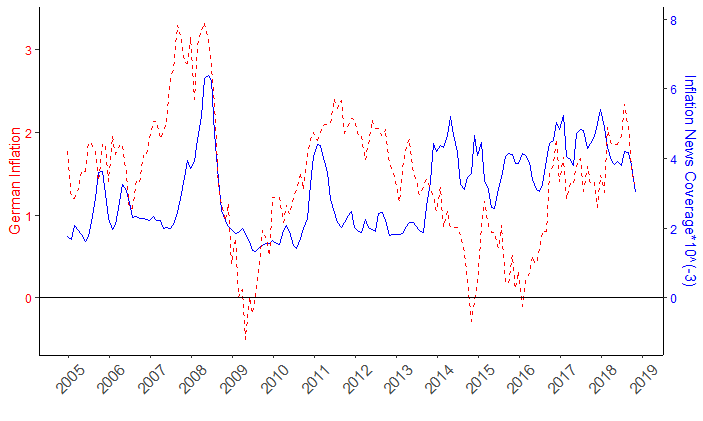
\includegraphics{Inflation_Count.png}
    \caption{Media Coverage}
    \label{10}
\end{subfigure}
\hfil
\begin{subfigure}{6cm}
    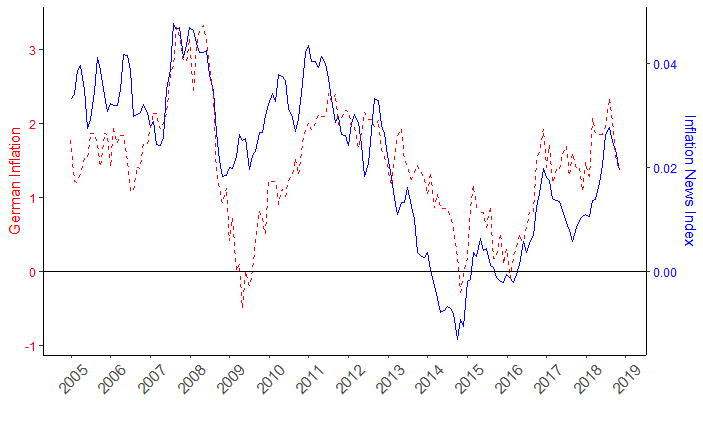
\includegraphics{Inflation_Sentiment_Direction.png}
    \caption{News Inflation Index}
    \label{100}
\end{subfigure}
\caption{Inflation and Media Reporting}
\label{fig:News Index}
    \end{figure}

\newpage    

\subsection{ECB Indexes}\label{sec:ECB Indexes}

\textcolor{red}{NOTE 1: Professional Forecaster Inflation Expectations are stronger correlated with ECB Inflation Index than with Inflation Expectations. Could be because of the European prof. Inf. Exp.}
\\
\textcolor{red}{NOTE 2: The results are quite similar to Picault et. al (2017) and Marozzi (2021), which is reassuring, but I only add 4 more years to the dataset. Therefore, my approach adds little new information regarding the ECB indices.}

   \begin{figure}[h!]
    \centering
    \setkeys{Gin}{width=\linewidth,height=6cm} %set image parameters
\begin{subfigure}{6cm}
    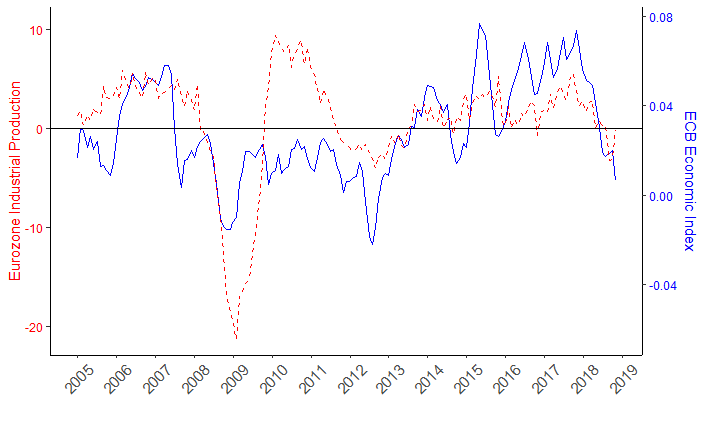
\includegraphics{ECB_eco_Industrial_prod.png}
    \caption{ECB Economic Outlook}
    \label{ECB_eco}
\end{subfigure}
\hfil
\begin{subfigure}{6cm}
    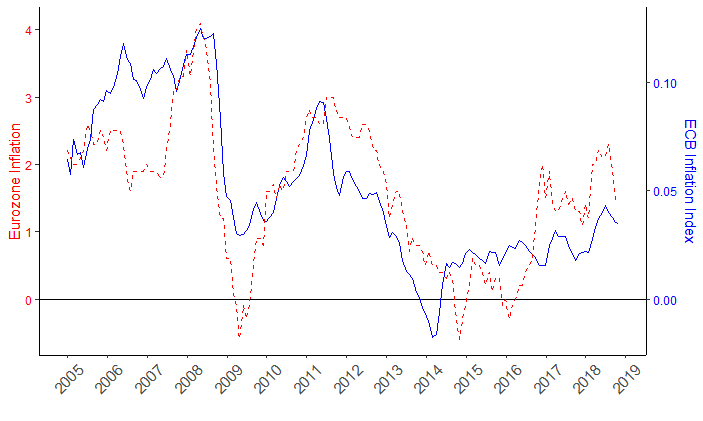
\includegraphics{ECB_inf_inf.png}
    \caption{ECB Inflation}
    \label{ECB_inf}
\end{subfigure}
\vfil
\begin{subfigure}{6cm}
    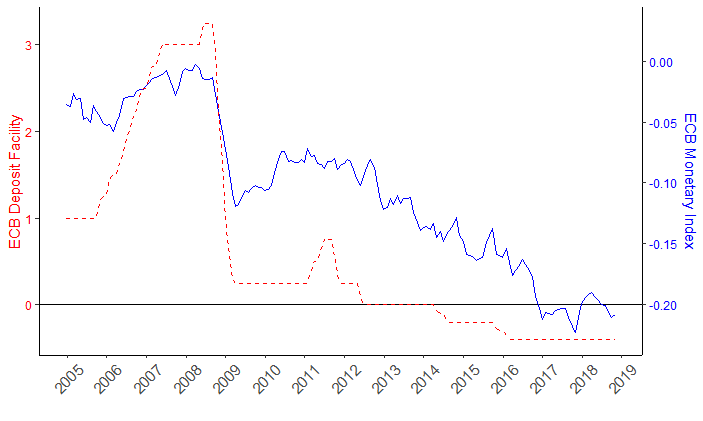
\includegraphics{ECB_mon_df.png}
    \caption{ECB Monetary}
    \label{ECB_inf}
\end{subfigure}
\caption{ECB Indices}
\label{fig:ECB Index}
    \end{figure}

\newpage

\subsection{Difference between ECB and News Indices (Placeholder title)}\label{sec:Difference between ECB and News Indices (Placeholder title)}

\cite{Carroll2003} define the inflation expectation error of households as the squared difference between the household inflation expectations and professional inflation expectations. \cite{LamlaLein2014} instead uses the absolute difference. Because I'm not only interested in the absolute size of the inflation gap, but also the direction 

To measure the error, I use the EU household inflation expectation described in and the professional inflation forecasts for the Eurozone described in (SECTION 2). My interest lies in the deviation between the household inflation expectations from the optimal forecasts. Therefore, I follow Lamla (2014) and calculate the household forecast errors as the difference between the household inflation expectations and professional inflation forecast for the Eurozone in the coming 12 months. I deviate from Lamla (2014) by taking the non-absolute error. (CITE) and (CITE) show that households react differently to news regarding high and low inflation.

\newpage

   \begin{figure}[h!]
    \centering
    \setkeys{Gin}{width=\linewidth,height=6cm} %set image parameters
\begin{subfigure}{6cm}
    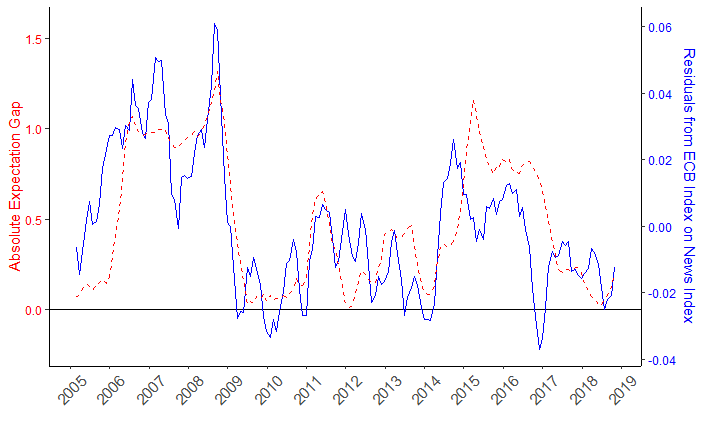
\includegraphics{abs_exp_res.png}
    \caption{Absolute Expt. Gap}
    \label{10}
\end{subfigure}
\hfil
\begin{subfigure}{6cm}
    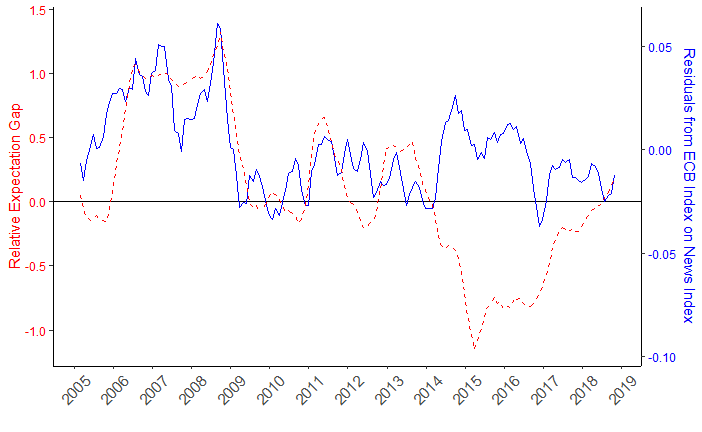
\includegraphics{rel_exp_res.png}
    \caption{Relative Expt. Gap}
    \label{100}
\end{subfigure}
\vfil
\begin{subfigure}{6cm}
    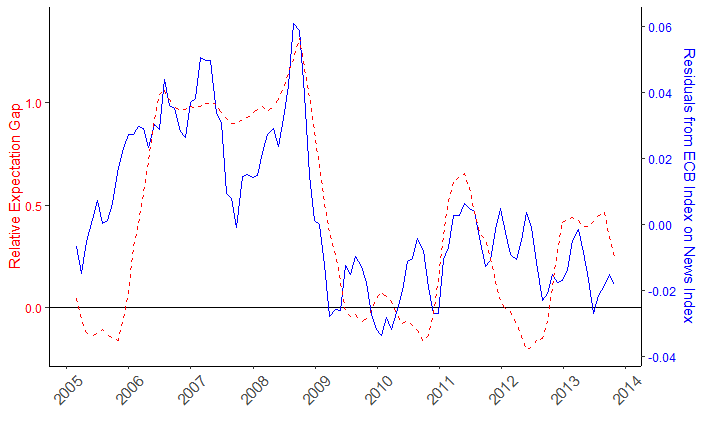
\includegraphics{rel_exp_res_prev2014.png}
    \caption{Relative Expt. Gap - Before 2014}
    \label{ECB_inf}
\end{subfigure}
\hfil
\begin{subfigure}{6cm}
    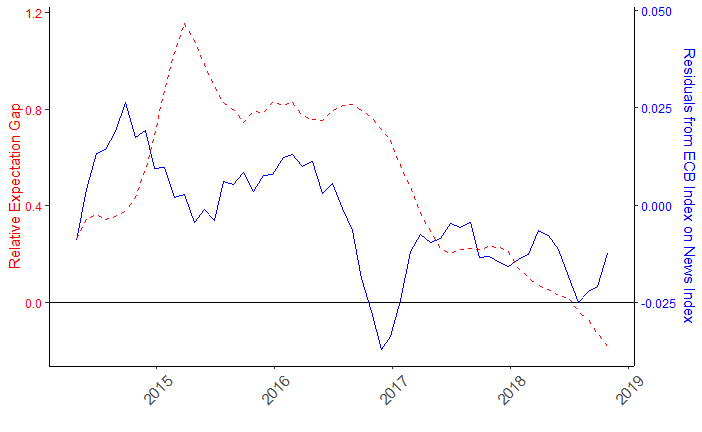
\includegraphics{rel_exp_res_aft2014.png}
    \caption{Negative Relative Expt. Gap - After 2014}
    \label{ECB_inf}
\end{subfigure}
\caption{ECB Indices}
\caption{Inflation Expectation Gap}
\label{fig:Expectation Gap}
    \end{figure}


\textcolor{red}{Lamla (2014) uses the absolute error. However, wouldn't it make more sense to take the non-absolute error in case of asymmetric behavior? Some papers indicate asymmetric behavior when it comes to inflation in news. Even if the behavior is symmetric, it could still be interesting to communicate that}
\\
\\
\textcolor{red}{How to continue from here? I probaly should define difference metric between the ECB inflation index and the news inflation index. Lamla (2014) simply do some OLS regression (Expecation gap on media indices. However, he also created a theorie which ties his regression together and lets him explain his results. I could try to modify his theory or come up with something on my own. Would that make sense???}

\section{Model}\label{sec:Model}

%$\pi^i_t$ = information regarding inflation which agents follow \\
$\pi^{ECB}_t$ = information regarding inflation from ECB \\
$\pi^n_t$ = information regarding inflation from news \\

$\epsilon_t$ = normal distributed error with mean zero and variance $\sigma_{ECB,t}$ \\
$\gamma_t$ = media bias \\
$\lambda_t$ = media bias weight (1 = full bias, 0 bias) \\

$\pi^{ECB}_t$ = $\pi^{Eurozone}_t + \epsilon_t$ (assuming that ECB is unbiased and focused on the Eurozone as a whole instead of country specific inflation.) 
\\
\textcolor{red}{Check if other papers made a difference for Eurozone inflation and country specific inflation.}
\\

$\pi^n_t$ = $\lambda_t * \pi^{ECB}_t + (1-\lambda_t) * (\gamma_t + \pi_t)$ (News can either follow ECB and just reproduce the ECBs press conferences ($\lambda_t = 1)$ or they could ignore the press conferences completely ($\lambda_t = 0$).) \\

%$\pi^i_t$ = $\alpha_t * \pi^{ECB}_t + (1-\alpha_t) * \pi^n$ \\
%$\pi^i_t$ = $\alpha_t * (\pi_t + \epsilon_t) + (1-\alpha_t) * (\pi_t + \lambda_t * \pi^{ECB}_t + (1-\lambda_t) * \gamma_t)$ \\
%$\pi^i_t$ = $\pi_t + \alpha_t * \epsilon_t + (1-\alpha_t) * (\lambda_t * \pi^{ECB}_t + (1-\lambda_t) * \gamma_t)$ \\

\subsection{Baysian Learning Framework}
% Einmal observed CB mit noise und dann kommuniziert es mit some noise. Da sollte ein noise raus 
\textcolor{red}{Baysian Framework from Kandel and Zilberfarb (1999) in Sheen and Wang (2022) and in Lamala and Lein (2014)}\\
\\
I assume that the central bank observes the true inflation $\pi_t$ with some noise. Let $c_t$ denote a measure that captures inflation-related information that the central bank communicates to the general public, i.e., inflation-related news in press conferences
\\
$ c_t = \pi_t + \epsilon_t \quad \epsilon_t \sim N(0, \sigma^c_t)$
\\ 
where $\epsilon_t$ represents the noise in the central bank's observation. 
\\
Without the central bank's communication, the media's "baseline" signal can be formulated as
\\
$ s^b_t = \alpha_t + \pi_t + \omega_t  \quad \omega_t \sim N(0, \sigma_t^{s^b}) $
\\
where $\alpha_t$ captures the media bias and $\omega_t$ is the noise. The media can decide how closely to follow the central bank's communication. Hence, the media's inflation signal can be defined as 
\\
$ s_t = \lambda_t s^b_t + (1-\lambda_t)c_t $
\\ 
where $\lambda_t$ denotes the weight that the media places on $s_t$. $\lambda_t = 1$ would indicate that the media ignores the central bank's communication completely and $\lambda = 0$ indicates that the media only reproduces the information from the central bank's communication. 
\\
Given that $s_t$ is a linear combination of normal random variables and assuming that $\epsilon_t $ and $\omega_t$ are independent the media sends a normally distributed signal $s_t \sim N(\mu_s, \sigma^s_t).$ 
\\
where 
\\$\mu_s = \lambda_t (\alpha_t + \pi_t) + (1-\lambda_t) \pi_t$ 
\\
$\sigma_t^s = \lambda_t^2 \sigma_t^{s^b} + (1- \lambda_t)^2 \sigma^c_t$
\\
The households hold a prior belief $\gamma_t \sim N(\pi_t, \sigma^h_t)$ about the future inflation $\pi_{t+1}$. Hence, the representative household forms its inflation expectations according to
\\
$ f(\pi_{t+1}|c_t, \pi_t, \lambda_t, \alpha_t) \propto  h(s_t|\alpha_t, \pi_t, \lambda_t) k(\pi_t)$
\\
where $f(\pi_{t+1}|c_t, \pi_t, \lambda_t, \alpha_t)$ is the posterior belief of a representative household on inflation $\pi_{t+1}$ after receiving the inflation related news signal. Assuming normality the posterior distribution can be represented as normal distribution with mean $\mu_t$ and variance $\vartheta_t$, where
\\
$ \mu_t = \rho \pi_t + (1 - \rho)(\lambda_t (\alpha_t + \pi_t) + (1-\lambda_t) \pi_t) $
\\
$ \mu_t = \rho \pi_t + (1- \rho) (\pi_t + \lambda_t \alpha_t)  $
\\
$\rho = \frac{\frac{1}{V}\sigma^s_t}{{\sigma^h_t + \frac{1}{V}}\sigma^s_t}$
\\
\frac{\partial }{•}
\\
For $\lambda_t = 0$ $\mu = \pi$. Hence, if the media perfectly reproduces the central bank communication, households would on average follow the current inflation for their expected inflation while $\lambda_t = 1$ would mean that media sends a signal which is biased by $\alpha_t$.  
\\
\textbf{Hypothesis 1:} If the media closely follows the central bank communication, households will be able to more directly follow inflation.
\\
\\
\textbf{Hypothesis 2:} If the media is strongly biased, 
\\
\textcolor{red}{Note: For a robustness check I could assume that households directly observe the ECB communication. Maybe I could even create a scenario in which the household ignore the media and only receive a news signal from the ECB, simulating a "perfect" communication scenario for the ECB.}  

\section{Econometric Framework}\label{sec:Econometric Framework}

I follow \cite{Erhmann2017} and define two different types of inflation expectation biases; $\mathbf{B}_t = \{B^r_t, B^e_t \}$ where $B^r_t$ is the difference between the HCPI and the transformed household inflation expectation at the forecast horizon, and $B^e_t$ is the difference between the professional inflation forecast and the transformed household inflation expectations.
\\
\textcolor{red}{to close to Erhmann et al. 2017?}
\\
$\mathbf{B}_t = \alpha + \beta_1 Media^c_t + \beta_2 Media^i_t + \beta_3 \pi_{t-1} + \epsilon_t$ \\

where $\alpha$ is a constant, 

%$Media^c_t$ is the news count in period $t$, $Media^i_t$ is the news inflation index  

The equation is estimated via OLS using Newey-West standard errors.
\\
To avoid simultaneity issues I follow \cite{LamlaLein2014} In order to obtain media data for a given month, I aggregate the media reports for each month, excluding any articles which are potentially related to the consumer survey results in the month. Specifically, I sum up the media articles until the day before the consumer survey is released. The sentences from the summed up articles are then used to derive the news index and news count for the given month.
\\
\textcolor{red}{Bezug zur Methode herstellen. Am besten Gleichung zitieren}
\\

\section{Estimation Results (Placeholder Title)}\label{sec:Estimation Results}

To understand how the media differs in their reporting about inflation compared to the official ECB communication, 

I measure the difference in inflation related news and inflation related ECB communication. 
To measure the difference of the ECB inflation index and the News Inflation Index 

\cite{LamlaLein2014} regressed professional forecaster inflation expectations on media 
\begin{align}
|\mu_{t+12} - \nu_{t+12}| = \alpha + |\mu_t - \nu_t| + \beta NewsInflation_t + \gamma ECBInflation_t + \mathbf{\delta} \mathbf{Z_t} + \epsilon_t
\end{align}

\begin{table}
\centering 
  \caption{Inflation Expectation Gap} 
  \label{tab:Inflation Expectation Gap}
\begin{tabular}{lcccccc}   
\\[-1.8ex]\hline
\hline \\[-1.8ex] 
& $Gap_{t+1}$ & $\mu_t$ & $\nu_t$ & & &\\ 
$Gap_t$ & & & & & &\\
$NewsInflation_t$ & & & & & & \\
$ECBInflation_t$ & & & & & &\\
$ECBMonetary_t$ & & & & & &\\
$ECBOutlook_t$ & & & & & &\\
$News ECB Difference_t$ & & & & & &\\
$Inflation_t$ & & & & & &\\
$IndustrialProduction_t$ & & & & & &\\
$Constant$ & & & & & &\\
\midrule
	$R^2$ & & & & & &\\
\bottomrule
 \end{tabular} 
\end{table}

\section{Conclusions} \label{sec:Conclusions}

%\section*{References}

\bibliography{mybibfile}

\newpage

\appendix

\section{Quantification of Inflation Expectations}\label{sec:Quantification of Inflation Expectations}

The European Commission's Business and Consumer Survey consumers are asked if they expect prices to fall, stay the same, increase slower than before, increase at the same rate or increase at a higher rate in the coming 12 months and in the last 12 months. 
\\
I use the rolling-window-regression approach by \cite{Lahiri2015} which is based on an extended version of the Carlson-Parkin method \citep{Carlson1975} by \cite{Berk1999}. The extended version of \cite{Berk1999} does not impose unbiasedness of inflation expectations. Instead the current perceived inflation rate is directly linked to the expected inflation rate.  
\\
By assumption each responded i forms a subjective probability distribution for individuals percentage price changes $y_{it}$ over the next twelve months. Let $f_i(y{_it})$ be the subjective probability distribution with mean $\mu_{it}$ and variance $\sigma_{it}$. Following \cite{Batchelor1988} method assumes for a survey with five possible answers that the respondent answers prices in the future increase, increase at the same rate, increase at a slower rate, stay the same or fall according as $ y_{it} < - \delta_{it}^L, - \delta_{it}^L < y_{it} < \delta_{it}^U , \delta_{it}^L < y_{it} < \delta_{it}^U,  \delta_{it}^U < y_{it} < \lambda_{it}, \lambda_{it} < y_{it}$ \textcolor{red}{Nochmal überprüfen, Ist Notation von \cite{Batchelor1988} besser?}. Based on the survey responses the corresponding aggregate probabilities can be formulated as $P(y <  -\delta_{it}^L) = A_t, P(y < \delta_{it}^U) - P(y > - \delta_{it}^L) = B_t, P(y < \delta_{it}^U) - P(y > \delta_{it}^L) = C_t, P(y < \lambda_{it}) - P(y > \delta_{it}^U) = D_t.$ I denote $a_t, b_t, c_t$ and $ d_t$ the abscissae of the standard logistical distribution function corresponding to the cumulative probabilities $A_t, \ A_t + B_t, \ A_t + B_t + C_t$ and $A_t + B_t + C_t + D_t$. The mean expected inflation rate $\mu_t = E_t \pi_{t+12}$ can then be formulated as 
\begin{align*}
\mu_t = \lambda_t \frac{(a_t + b_t)}{(a_t + b_t - c_t - d_t)}
\end{align*}
Similarly, I denote $a_t\sp{\prime}, b_t\sp{\prime}, c_t\sp{\prime}$ and $ d_t\sp{\prime}$ as the abscissae of the standard logistical distribution function for the perceived inflation. Assuming that the response threshold $\lambda_{it}$ \textcolor{red}{Nochmal überprüfen} is the same for expected and perceived inflation, the perceived inflation can be formulated as 
\begin{align*}
\mu_t\sp{\prime} = \lambda_t \frac{(a_t\sp{\prime} + b_t\sp{\prime})}{(a_t\sp{\prime} + b_t\sp{\prime} - c_t\sp{\prime} - d_t\sp{\prime})}
\end{align*}
For the choice of the scaling parameter $\lambda_t$ I use the rolling window based regression by \cite{Lahiri2015}. Following \cite{Rosenblatt-Wisch2015} running the regression
\begin{align*}
\pi_t = \lambda \frac{(a_t\sp{\prime} + b_t\sp{\prime})}{(a_t\sp{\prime} + b_t\sp{\prime} - c_t\sp{\prime} - d_t\sp{\prime})} + u_t 
\end{align*}
using a sample window of $t - w + 1 to t$ implies
\begin{align*}
\hat{\lambda_t} = \frac{\sum^t_{k = t-w+1}(a_t\sp{\prime} + b_t\sp{\prime})/(a_t\sp{\prime} + b_t\sp{\prime} - c_t\sp{\prime} - d_t\sp{\prime})\pi_t}{\sum^t_{k = t-w+1}(a_t\sp{\prime} + b_t\sp{\prime})/((a_t\sp{\prime} + b_t\sp{\prime} - c_t\sp{\prime} - d_t\sp{\prime}))^2}
\end{align*}
where $w$ is the size of the rolling window. \cite{Lahiri2015} choose $w$ as nine years for the inflation expectations of the Michigan Consumer Survey. I follow \cite{Lahiri2015} and also choose nine years for $w$. The resulting household inflation expectations and the professional inflation expectations are shown in figure~\ref{fig:Inflation Expectations}.
\\
\textcolor{red}{Robustness Check for different windows?}
\\
\textcolor{red}{TO CLOSE TO Rosenblatt-Wisch and Scheufele 2014??}

  \begin{figure}[h!]
    \centering
    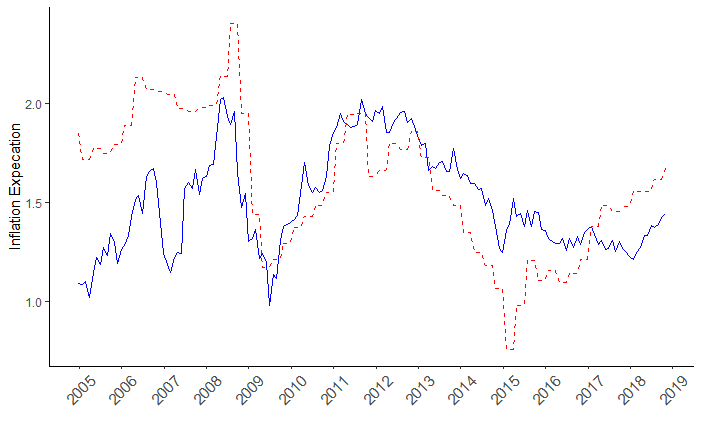
\includegraphics[width=\linewidth,height=6cm]{household_prof_inf.png}
    \caption{Inflation Expectations: Household inflation expectations are in blue, Professional forecaster inflation expectations are in red}
    \end{figure}
\label{fig:Inflation Expectations}

\section{Additional Rules for Lexicon Text Classification}\label{sec:Additional Rules for Lexicon Text Classification}

\end{document}